\section{Architecture}
\label{sec:arch}

An AsyncBTree tries to achieve better performance compared to a conventional binary tree and binary fat tree in terms of resource utilization and throughput by applying FPGA and topology specific optimizations and using asynchronous links between different tree levels.
Fig.~\ref{fig:btree} shows the architecture of an AsyncBTree utilizing different kind of optimized switches at different levels.
The detailed architecture of the switches are discussed in Section~\ref{sec:switch}.
The binary tree is placed and routed in the FPGA as an H-tree for efficient resource utilization and better floor-planning.
Such placement also supports partial reconfiguration of a portion of the NoC in an efficient manner.
As the first optimization, the root node of the tree is removed and the switches at level-1 are directly connected.
Since the connectivity of the root node is only 2, in practical systems they act as a transparent switch.
They could be useful where packets are injected to the NoC through the root node by making its connectivity into 3.
For FPGAs external interfaces such as PCI express and Ethernet are used for injecting packets.
The hard-macros corresponding to these interfaces are situated along the periphery of the chips.
Thus it will provide better clock performance when the packets are injected from one the leaf nodes which incorporates one of these hard macros.
Removing the root node helps in reducing the resource utilization.

\begin{figure}[t]
\centering
   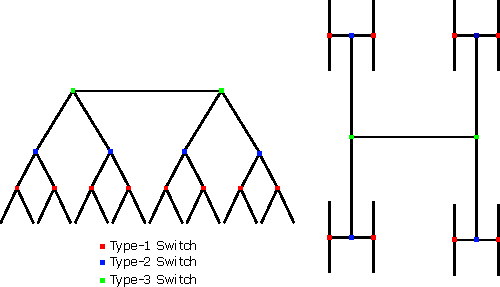
\includegraphics[width=\columnwidth]{Figures/HNoC.pdf}
   \caption{(a)A binary tree topology utilizing switches operating at different clock frequencies (b) The tree as an H-tree for better floorplanning on the FPGA}
   \label{fig:btree}
\end{figure}

\begin{figure}[t]
\centering
   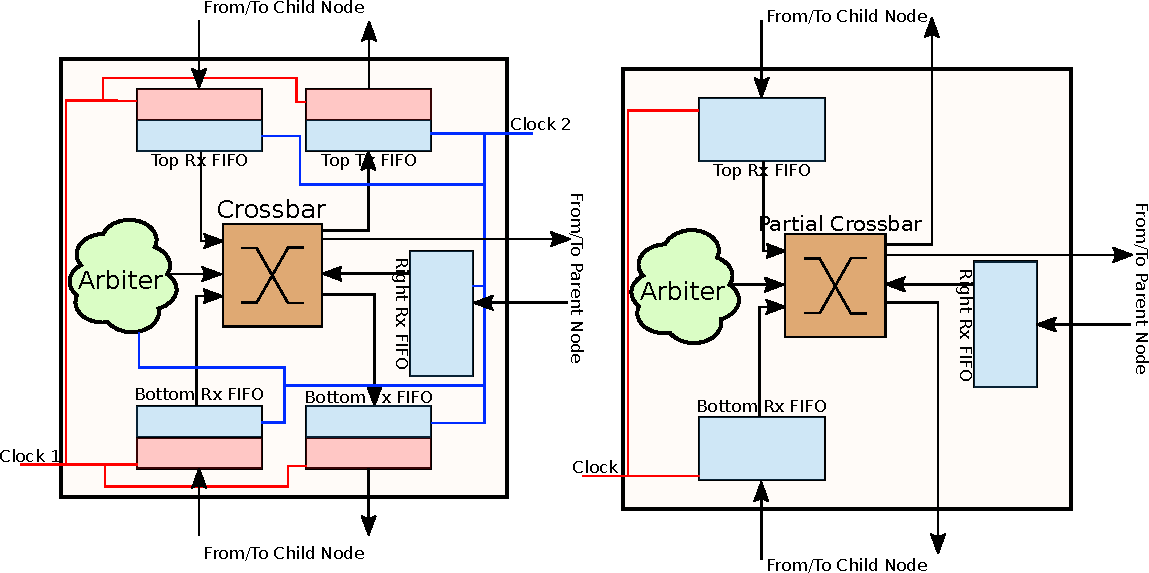
\includegraphics[width=\columnwidth]{Figures/switch1_2.pdf}
   \caption{Architecture of the different switches used in the AsyncBTree. (a) Type-1 switch used with the leaf nodes (PEs), with complete cross bar switch and asynchrnous 
   FIFOs with receive and transmit interfaces (b) Type-2 switch used in intermediate nodes with partial crossbar switch and synchronous FIFOs (c) Type-3 switches used in intermediate
   switches with partial cross bar and asynchrnous FIFOs with receive and transmit interfaces.}
   \label{fig:switchArch}
\end{figure}

\subsection{Switches}
\label{sec:switch}
AsyncBTrees use three different kinds of switches for packet routing.
The architecture of the proposed type-1 switch is as shown in Fig.~\ref{fig:switchArch}(a).
Type-1 switches are used only in the leaf nodes for directly interfacing with PEs.
The switch has separate interface for receiving and transmitting packets from two PEs and a single interface to the parent node.
Each receive and transmit interface to/from the PEs are connected to asynchronous FIFOs.
The interface to the parent node implements a single synchronous FIFO for the receive interface but no transmit FIFO.
Thus each switch contains 5 FIFOs.

Asynchronous FIFOs can operate their read and write interfaces using independent clocks.
Depth of the FIFOs are kept very low (16) to reduce the resource utilization.
The asynchronous FIFOs receive data from the downstream ports on Clock 1 signal.
The received packets are routed to the appropriate output ports by an arbitrator through a cross-bar switch.
The read side of the receive FIFO, the write side of the transmit FIFO, the arbitrator and the cross bar works on Clock 2 signal, whose frequency will be much higher than that of Clock 1.
In order to match the performance of a binary fat tree, Clock 2 frequency should be twice as that of Clock 1.

Type-1 switches implement a full cross bar, which enables loop back of packets at the switch level.
The arbitrator internally uses flit-level round-robin arbitration scheme to select the input port when more than one port requests for the same output port.
If a single input port is requesting for a particular output port, it is given the port access until all the flits are sent out.

Fig.~\ref{fig:switchArch}(b) shows the architecture of a type-2 switch.
Type-2 switches are synchronous in nature and are similar to the switches of traditional binary trees.
These switches implement only partial cross-bar switch where an in coming packet cannot be routed back to the same port.
Since these switches are used only in intermediate levels, there is no necessity to to support loop-back since they are already implemented by Type-1 switches.
This simplifies the switch design and helps in reducing resource utilization.

Type-3 switches (Fig.~\ref{fig:switchArch}(b)) are similar to type-1 switches except that they implement only a partial cross-bar similar to type-2 switches.
Type-2 and type-3 switches can be interchangeably used in the proposed architecture. 
Theoretically to match the performance of a binary fat tree, AsyncBTrees should be implementing type-3 switches at every level with increasing clock frequencies.
But in practical scenarios, doubling clock frequency at each level is not possible in FPGAs as the tree size increases.
The maximum frequency supported by modern devices are in the order of hundredes of megahertz.
Hence for practical implementations, AsyncBTrees increases the clock frequency only for alternative levels. 
Although asynchronous FIFOs can operate using same clock signal for read and write interfaces, the resource utilization of an asynchronous FIFOs is much more than its synchronous counter part for a given FIFO size.
It is because of the presence of additional circuitry for managing clock domain crossing between the read and write interfaces.
For reducing resource consumption, levels which operates on synchronous clock uses type-3 switches and levels which operate on asynchronous clock uses type-2 switches.

\subsection{Routing}
\label{sec:routing}
AyncBTree uses fixed routing based on the destination address of the packet header~\ref{fig:packet}.
The routing is flit level routing meaning each packet is expected to have the destination PE address in the packet header.
Larger packets are sent as multiple flits.
One major advantage of binary trees is the multiple packets sent from one PE to another will be always delivered in the sent order.
In other packet switched networks such as mesh or torus, the packets could be delivered in out of order depending on the routing algorithms.
In this case additional logic is required for packet reassembly and packet numbers also have to be inserted into the payload.

The routing table of each switch in AsyncBTree contains four entries corresponding to the smallest and largest PE addresses in its left sub-tree and right sub-tree.
If the destination address is with in the range of left sub-tree, it is routed left and if it is with in the range of right sub-tree the packet is sent right.
If the address is not within these ranges, the packet is routed towards the parent node.
Due to the deterministic routing policy and since the routing is at flit-level, the NoC is free of dead or livelocks.

\begin{figure}[t]
\centering
   
\includegraphics[width=\columnwidth]{Figures/pckt_structure.pdf}
   \caption{Packet structure}
   \label{fig:packet}
\end{figure}

\section{Flow control}
The current AsyncBTree implementation does not include virtual channels and flow control is achieved through at electrical signaling level.
The interface between switches as well as switches and PEs confirm to AXI4-stream interface.
Such interface also enables seamless integration of several vendor supported IP cores directly with the NoC.
As per AXI4-stream protocol, a successful data transfer happens only when the \emph{valid} signal from the transmitter and \emph{ready} signal from the receiver are asserted as shown in Fig.~\ref{axi}.